\documentclass[a4paper]{article}
\usepackage{fullpage}
\usepackage[english]{babel}
\usepackage[utf8]{inputenc}
\usepackage{amsmath}
\usepackage{graphicx}
\usepackage{enumitem, mdwlist }
\usepackage{mathbbol}
\usepackage{float}
\usepackage{amssymb}
\usepackage{multirow}
\usepackage{array}
\usepackage{minted}
\usepackage{esvect}

\title{The Ising Model of Ferromagnetism }

\author{Computational project: Dr. David Buscher}

\setlength{\parskip}{1em}

\date{\today}

\begin{document}
\maketitle

\begin{abstract}

The time evolution of the mean magnetisation $ \langle M \rangle $ per spin was investigated for a range of temperatures and initial conditions. The temperature dependence of the mean energy $ \langle E \rangle $ and mean absolute magnetisation $ \langle |M| \rangle $ was determined. The latter is used instead of normal magnetisation to avoid the complications of spontaneous magnetisation at low T. The heat capacity C was also plotted as a function of T using both a discrete derivative and the fluctuation dissipation-theorem. The Curie temperature is estimated graphically from these plots, $T_c = 2.29 \pm 0.03$, as the temperature at which the phase transition occurs and compared with Onsanger analytical result. Lastly, a finite size scaling analysis is undertaken to determine the critical exponent $\beta = 0.126 \pm 0.006$. The ferromagnetic response to an external magnetic field $H$ is also analysed. A copy of the source code used is joined in the appendix.


\end{abstract}


\section{Introduction}

Unlike ordinary materials, ferromagnets can display a preferred spin alignment, resulting in a net dipole moment. This macroscopic effect depends on the thermodynamic properties of the system and on external magnetic fields. The Ising model allows us to calculate the ferromagnetic properties, like the magnetisation $M$, the energy $ E $ and the heat capacity $C$ of the system as a function of temperature. There are two main principles affecting the spin configuration, \textit{energy minimization} and \textit{entropy maximization} of the system. These factors have opposite contributions and are described by the Boltzmann probability, $ p = exp(-\beta E) $. The inverse temperature T, $\beta, (in units of k, the Boltzmann constant)$, is fixed by a heat bath. If brought in contact with it, the individual spins of the material will flip back and forth, exchanging energy until a thermal equilibrium is reached. This report is a study of the properties of ferromagnetic materials using a self-written Monte Carlo code for the two-dimensional Ising model. The aim is to test the validity of the Ising model by evaluating the observables of a ferromagnet. Key background is given about the Monte Carlo stochastic approach and the applicability of the Metropolis algorithm. The computational aspects of the problem, and in particular the steps taken to make the program run efficiently, such as the pre-calculation of the Boltzmann factors, are then analysed. We then discuss the measurement of observables and compare to exact calculations to test the validity of the numerical methods.

\pagebreak



\begin{table}
\centering
\begin{tabular}{l|c|c|c}
\hline
 &  $x_P$ [GeV] &  $\sigma_P$ [GeV] & Asymmetry $\xi$ \\
\hline
Nominal     & $551 \pm 7$       & $63 \pm 5$           & $-0.30 \pm 0.08$  \\                    
REG         & $569 \pm 7$       & $58 \pm 4$           & $-0.29 \pm 0.08$  \\                   
FSR         & $555 \pm 7$       & $63 \pm 5$           & $-0.29 \pm 0.08$  \\                 
REG+FSR     & $574 \pm 6$       & $57 \pm 4$           & $-0.30 \pm 0.07$  \\
               
\hline
\end{tabular}
\caption{ Semi-leptonic }
\end{table}
\vspace{0.1cm}


\pagebreak

\section{Analysis of the computational physics}

\subsection{Background theory}

The simplest formulation of an atomic magnetic moment is provided by the Ising spin $s_i$. In two dimensions, the spin is either aligned or anti-aligned with the z axis ($s_i = \pm 1$). Let us consider a square array of $N = L$ x $L$ spin sites. Since the magnetic dipole interactions fall off with $r^{-3}$, we are only interested in nearest-neighbour spin interactions (Fig.1). The interaction energy for a specific spin site is:

\begin{equation}
E = -J \sum_{\substack{ \langle ij \rangle}}s_i s_j -\mu H \sum\limits_{i = 1}^N s_i
\end{equation}



where $J$ is the exchange energy, $\mu$ the magnetic moment, and $H$ the applied magnetic field. The coupling constant $J$ determines the nature of the spin interaction. If positive, the material is ferromagnetic, i.e. it favours parallel spin alignment with $s_i s_j = +1$. If negative, the system is antiferromagnetic. A further simplification is that we measure the energy in units of $J/k_b$ and we set $\mu$ to unity. The external field $H$ couples to the magnetisation of the system calculated as:
\begin{equation}
M =  \sum_{\substack{i}}s_i
\end{equation}

The spins tend to align with the external magnetic field. If there is no applied field, the system can exist in two distinct phases depending on the temperature \cite{stat}. At low temperatures, the system is permanently magnetised, while at sufficiently high ones, the system has no net magnetisation. The critical temperature $T_c$ marks the phase transition between the ferromagnetic and the paramagnetic phases. The Ising model is defined in the limit for an infinite lattice size L. To compensate for finite L, we can maximise the interaction between the spins at the edge of the lattice by requiring them to interact with the spins at the geometric opposite edge. This arrangement is referred to as periodic boundary conditions, and it can be visualised by folding the 2d lattice into a 3d torus (Fig.2).


\begin{figure}[h]
\centering
\begin{minipage}[b]{0.3\linewidth}
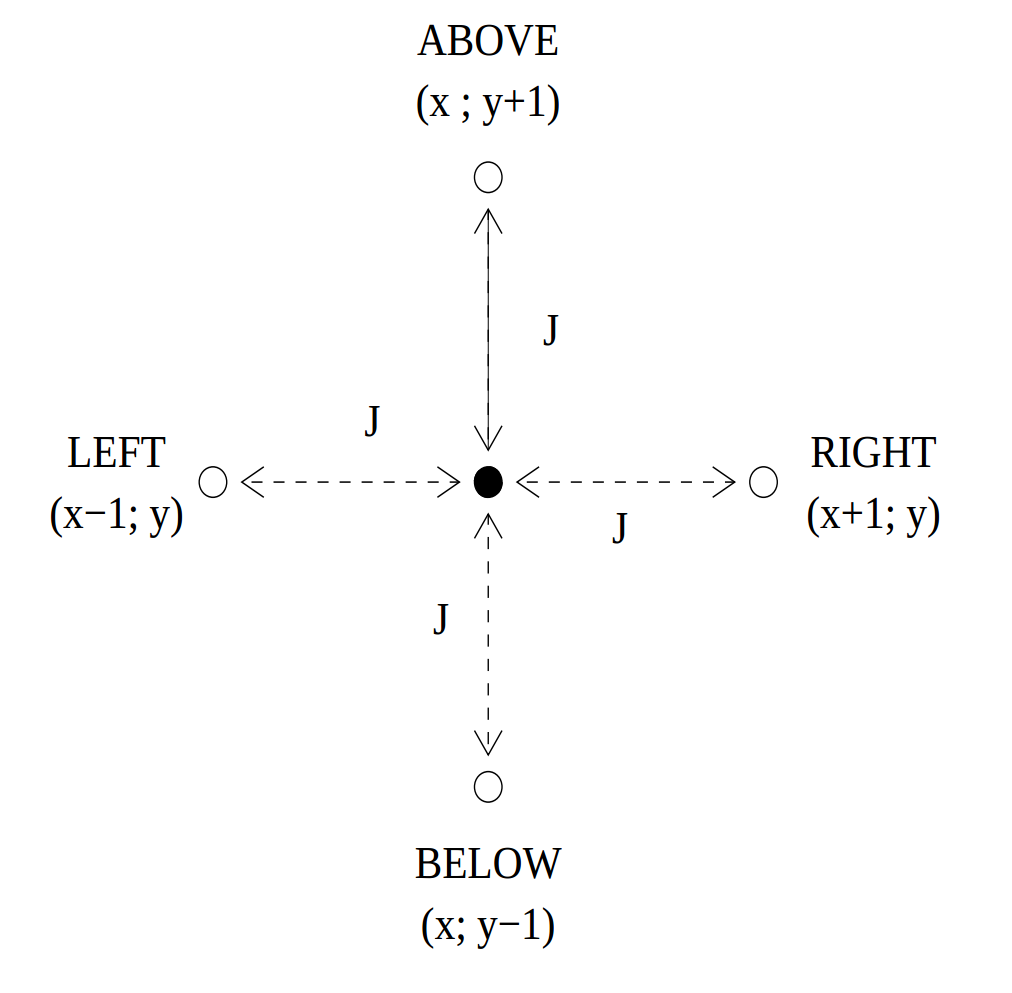
\includegraphics[width=1\textwidth]{neighbour.png}
\label{fig:minipage1}
\caption{An illustration of next neighbour coupling interactions for a single spin site.}
\end{minipage}
\hspace{1.85cm}
\quad
\begin{minipage}[b]{0.4\linewidth}
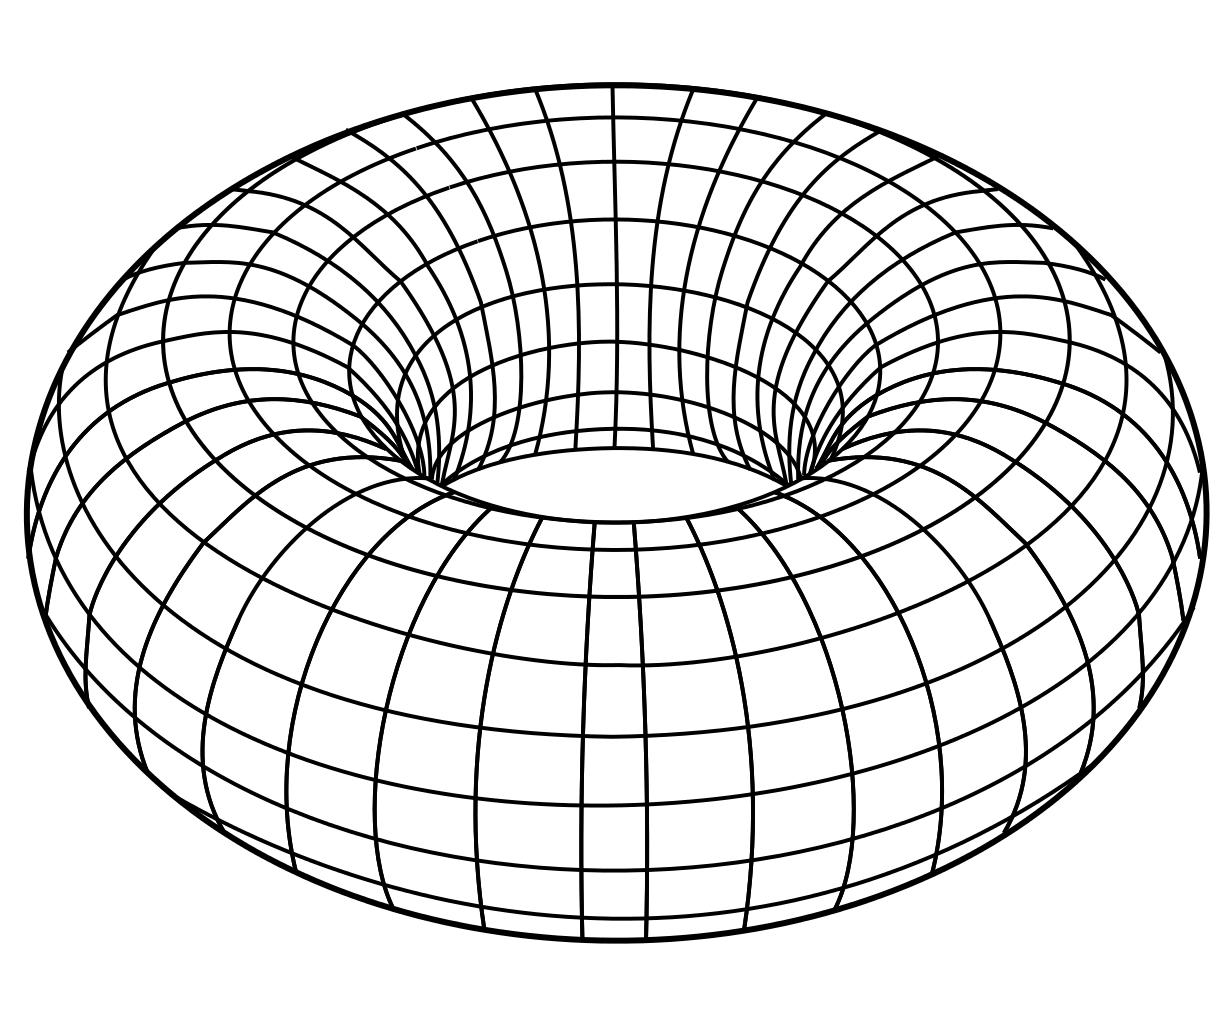
\includegraphics[width=1\textwidth]{torus.png}
\label{fig:minipage2}
\caption{The torus topology representative of the periodic boundary conditions (pbc) in a planar spin lattice.}
\end{minipage}
\end{figure}


\subsection{Monte Carlo simulation}

Monte Carlo simulations involve generating a subset of configurations, chosen using a random algorithm from a \textit{configuration space}, according to a probability distribution\cite{mcs}. In our case, the sample is a particular spin assignment, in which each spin is either "up" or "down". According to statistical mechanics, we can compute the mean value of the ferromagnetic observable A for some temperature by weighting each configuration with the Boltzmann probability:

\begin{equation}
\langle A \rangle = \frac{\sum_{\substack{ configs}} A e^{-E/kT}}{\sum_{\substack{ configs}}  e^{-E/kT}}
\end{equation}

If the number of configurations $M$ tends to infinity, this equation reduces, as expected, to the \textit{thermodynamic average} for a canonical ensemble with partition function $Z$:

\begin{equation}
\langle A(x) \rangle_T = \frac{1}{Z} \int e^{-\beta H(x)}A(x)\, \mathrm{d}x \hspace{1cm}  with \hspace{1cm} Z = \int e^{-\beta H(x)}\, \mathrm{d}x
\end{equation}

\vspace{2cm}


\begin{equation}
f(M_{12})  = \frac{1}{2} Erf(p_0(M_{12} -p_{1}) + 1 ) \hspace{0.5cm} with \hspace{0.5cm} Erf(x) = \frac{2}{\sqrt[]{\pi}} \int_{0}^{x}  e^{-t^2}\, \mathrm{d}t
\end{equation}

In theory, we calculate the observables using (3). However, the total number of possible configurations of the system increases as $2^N$, which is intractable even for a moderate lattice size. For instance, for $L = 20 $, $N = 400$, the total number of microstates becomes $\sim 10^{120}$. Even a very fast processor, evaluating a billion configurations per second, would need more than $10^{103}$ years to compute the average magnetisation exactly. A smarter sampling technique is to focus on the most representative states, also called \textit{importance sampling}. In a Monte Carlo simulation, we generate a reasonable number of random configurations. Then the probability of a particular configuration (a representative point in phase space) is given by its Boltzmann factor divided by a suitable weight function:

\begin{equation}
 p(s_1, s_2, ..., s_N) = \frac{e^{-E(s_1, s_2, ..., s_N)/kT}}{\sum_{\substack{ configs}} e^{-E/kT}}
\end{equation}

It can be shown that by weighting the terms being summed in equation (3) with this probability, the Boltzmann factors cancel out. Observables can then be calculated by performing arithmetic averages of the spin configurations. Sampling is analogous to a time averaging along a stochastic trajectory in phase space. Therefore, we can treat the single Monte Carlo steps (mcs) as a unit of time. 

\begin{equation}
\langle A(x) \rangle = \frac{1}{N} \sum_{i=1}^{N} A(s_1, s_2, ..., s_N)
\end{equation}


\subsection{Calculation of observables}

The observables of interest are $\langle E \rangle$, $\langle E^2 \rangle$, $\langle M \rangle $, $\langle M^2 \rangle$ and can be calculated using (6) in the following way:

\begin{equation}
\langle M \rangle = \frac{1}{N} \sum_{i=1}^{N} M
\end{equation}

To calculate the energy, we need to account for correct counting of the spins. The error estimate is purely statistical. At Curie temperature, there is a marked fluctuation in these quantities. We can compute the heat capacity both in a discrete form, using the ratio of successive energy steps by the temperature step,

\begin{equation}
C = \frac{\partial E}{\partial T} \approx \frac{E(T+ \delta T)- E(T)}{\delta T} 
\end{equation}

or more accurately with the fluctuation dissipation theorem and ${\sigma_E}^2 = \langle E^2 \rangle - {\langle E \rangle}^2 $. 

\begin{equation}
 C   = \frac{{\sigma_E}^2}{kT^2} = \frac{\langle E^2 \rangle - {\langle E \rangle}^2}{kT^2} 
\end{equation}


\subsection{Metropolis-Hastings algorithm}

An ingenious algorithm to generate random, Boltzmann distributed configurations was discovered by Metropolis \textit{et al} \cite{met}. This algorithm prescribes a detailed balance between two states in thermodynamic equilibrium. The equation relating the transition rates $W$ between the states $x_i$ and $x_j$ at equilibrium is:  

\begin{equation}
p_{eq}(x_i)W(x_i \rightarrow x_j) = p_{eq}(x_j)W(x_j \rightarrow x_i)
\end{equation}

The ratio of the probabilities only depends on the energy difference $\Delta E$ since

\begin{equation}
\frac{W(x_i \rightarrow x_j)}{W(x_j \rightarrow x_i)} =  e^{-\Delta E/kT}
\end{equation}

 
In our simulation, the Metropolis algorithm is implemented in the following way:
\begin{itemize}
\item The spin system is initialised in a particular microstate. This might either be a homogeneous or random configuration. A random configuration has the benefit that it uses less computing time to reach the equilibrium state.
\item A spin site is selected randomly. This could also be done in a sequence but is avoided  not to bias the sample.
\item The energy change of the system $\Delta E$ is computed.
\item Let the ratio of the transition rates be $w = exp(-\Delta E/kT)$. If $w > r$ where r is a uniform random deviate between 0 and 1, the spin is flipped, otherwise no change. Note that this instruction also implies that the spin must always flip for $\Delta E < 0 $ in accordance with the principle of energy minimization. 
\item The steps listed above are repeated for N spins in the configuration to complete a single Monte Carlo time step.
\item All the steps are repeated for a single Monte Carlo loop. Once the loop is completed for a fixed value of T, we are left with the sum of all the spin configurations generated within the loop. We can recover and store the relevant thermodynamic variables by averaging over the total accumulated change in the observables.
\end{itemize}


This sequence produces the observables for a specific temperature. In the main program \verb;ising.cc; we introduce a temperature loop with step size $\delta T$, while in \verb;ising2.cc; we implement an analogous loop for the magnetic field $H$. The different lattice sizes considered were $L = 2^k$ for integer $k \leq 4 $. After the initialization of the equilibrium, the system will be most likely not in thermal equilibrium with the heat bath. The preliminary Monte Carlo steps required to thermalise the system are called transients and should be discarded from the calculations. 

\section{Implementation and optimisation of the code}

Both programs can be compiled using \verb;g++ -Wall ising.cc -o ising.exe -lgsl; \verb;-lgslcblas -lm; and including the header file $<$\verb+gsl/gsl_rng.h+$>$. The function \verb;double rand_uniform(); uses a standard gsl routine to calculate a random deviate in the interval $[0;1]$. 

\subsection{Calculation of the observables}

The observables calculated in \verb;ising.cc; are $\langle E \rangle$, $\langle E^2 \rangle$, $\langle M \rangle $, $\langle |M| \rangle$ and $C$. The energy and magnetisation functions compute the mean magnetisation and energy per spin using pbc. To avoid double spin counting, an efficient solution is to sum only over two neighbouring spins (i.e. the top and right one) for each spin site. In the main loop, we take averages of the total sum of each variable to calculate the observables. The random errors in $\langle M \rangle $ and $\langle E \rangle$ are approximated using the error formula ${\Delta A}^2 = \langle A^2 \rangle - {\langle A \rangle}^2 $ and weighted by $\sqrt mcs$. The error in C calculated with equation (8) is negligible and overly complicated to compute. The random error in (9) is calculated by adding in quadrature the errors in the energy terms $E(T+ \delta T)$ and $E(T)$ and dividing by $\delta T$. 


\subsection{Spin configuration }

The spin configuration is initialised with \verb;initialise(); which sets four possible starting conditions: \verb;up;  \verb;down; (homogeneous spin configurations), \verb;warm; (randomly aligned spins) and \verb;hot; (neighbouring spins anti-aligned). The spin configuration can be visualised with \verb;print_spin_config(); which prints out a binary matrix corresponding to the $s_i = \pm 1$ values, which was plotted with gnuplot. Only a thousand transient steps are required, resulting in a more efficient thermalisation. This was achieved by initialising the configuration at the start of each temperature or magnetic field step using the previous one, and using a small $\delta T = 0.1$.

\subsection{Metropolis and Monte Carlo steps }


A randomly chosen spin $s_i$ is such that $s_{i,trial} = -s_i$. The energy change in the system is given by
\begin{equation}
\Delta E = E(s_1, s_2,..., s_{i,trial}, ...,s_N) - E(s_1,s_2, ...,s_i, ..., s_N)
\end{equation}

hence for a single spin $\Delta E = -2E(s_i)$. If $w > r$ then flipping occurs ( $s_{i,trial} \rightarrow s_i$). If we did not precompute the Boltzmann factors, we should have added a preliminary if statement to check whether $\Delta E <0 $. In this case, flipping must always occur, making the calculation of a Boltzmann factor redundant. However, precomputing the Boltzmann factors eliminates any additional cost. In fact, this is a more compact and efficient statement. If the spin site is at the edge of the lattice, pbc are used to determine its neighbours. A single Metropolis step will yield a highly correlated configuration with the previous one. In Monte Carlo simulations, it is conventional to take N Metropolis steps to generate the next configuration, such that each spin has the chance to change its state. 
 
\subsection{Efficient evaluation of Boltzmann factors}

The exponential factor $w = exp(-\Delta E/kT)$ is expensive to compute for each Metropolis step. By inspection, it can be shown that for a fixed value of $T$ and $H$ (a single step of the temperature or magnetisation loop), there are only ten distinct values for w. Pre-computing these ten values at the start of each step, saves the expense of $N_t$ = $N$ x $mcs$ calculations (of the order of several millions). The sum of the neighbouring spins of a spin site gives 

\begin{equation}
\sum_{\substack{ neighbours\hspace{1.5mm} j}} s_j = +4,+2,0,-2,-4
\end{equation}

i.e. $+4$ if they all point up, $+2$ if three point up and one down, etc. Since  $s_i = \pm 1$, the product of $s_i$ with the sum takes the same set of five values. If $H \neq 0$ the energy term $H s_i$ takes the values $\pm 1$. Thus, in general, there are ten distinct values for w.
\begin{verbatim}
void calc_Boltzmann_factors ( double& T ) {
     for (int i = -8; i <= 8; i += 4) {
          w[i + 8][0] = exp( - (i * J + 2 * H) / T);
          w[i + 8][2] = exp( - (i * J - 2 * H) / T);
     }
}
\end{verbatim}
The indices of a c\scriptsize{++} \normalsize array must be non-negative. The second index for $H$ values of $w$[ ][ ] is $1+s_i = 0,2$, and the first index is

\begin{equation}
8 + 2 s_i \sum_{\substack{ neighbours \hspace{1.5mm} j}} s_j = 0,4,8,12,16
\end{equation}


\subsection{Performance}

The computation times for different lattice sizes of a whole temperature loop from $T = 0.5$ to $5$ K with step size $\delta T = 0.05$ were compared in Fig.3.
The simulation was run with a hundred thousand mcs and a thousand transient steps. As expected, the computation cost is directly proportional to the total number of spins $N$ and to the number of mcs.

\begin{figure}[H]
\centering
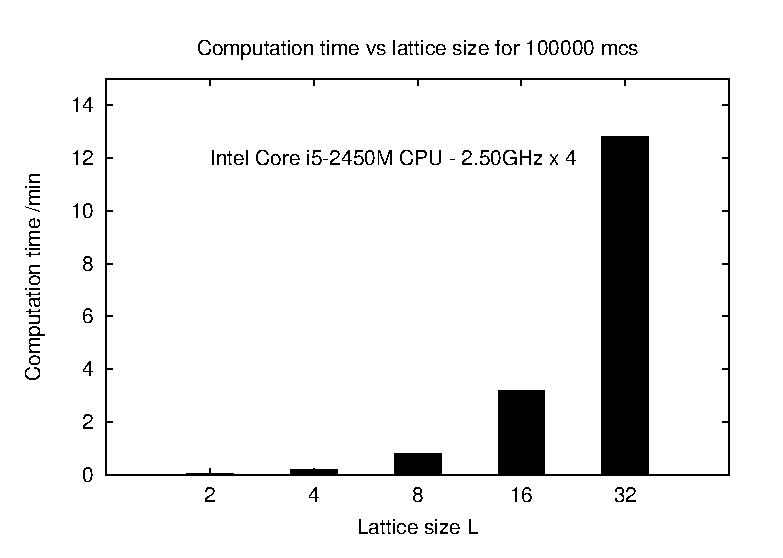
\includegraphics[width=0.51\textwidth]{histogram.eps}
\caption{This plot illustrates how computation time varies with lattice size L. The processor used was an Intel Core i5-2450M CPU @ 2.50GHz x 4.}
\end{figure}

 
\section{Results and Discussion}
\subsection{Testing the program}

The main program was tested using a random initial spin configuration and $H = 0$. The configurations evolve differently according to the ferromagnetic ($T < T_c$), or paramagnetic ($T > T_c$) phase. The long term behaviour in the low and high temperature limit was checked to agree with theory. We initially choose a very large $L = 500$ as the model is defined in the thermodynamic limit $L \rightarrow \infty$, and let the system evolve. In the ferromagnetic regime for $T = 0.1$, domain formation occurs after just 100 mcs (Fig.4). According to theory, all the spins will tend to be aligned in the ferromagnetic case. In Fig.5, a metastable state is seen with two  regions with the dominance of a single spin. At intermediate temperatures $T = 3K > T_c$ the net magnetisation of the system converges rapidly to zero ($\langle m \rangle = 0.022 \pm 0.004$ even just after 100 mcs). The resulting random spin alignment is consistent with paramagnetism (Fig.6). For high temperatures T = 10 K, both the theoretical and average acceptance ratio of the spin flip tends to one. The neighbouring spins tend to anti-align in a checkerboard pattern (Fig.7). 

\vspace{3mm}

\begin{figure}[h]
\centering
\begin{minipage}[b]{0.45\linewidth}
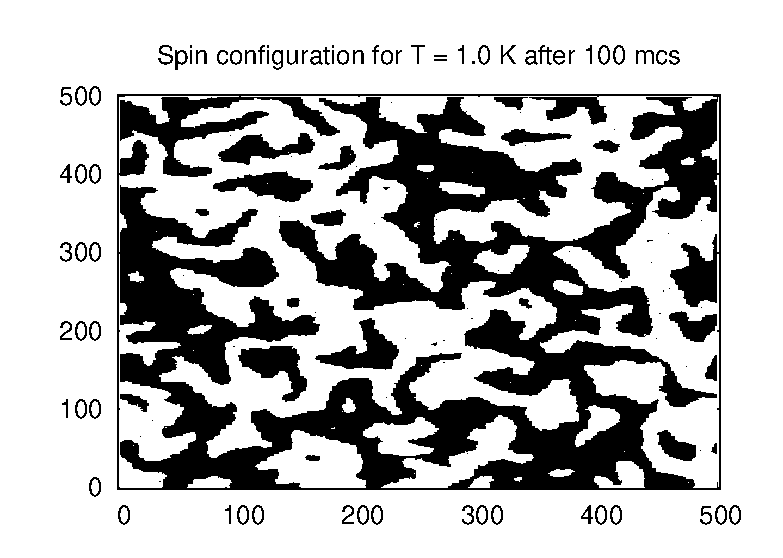
\includegraphics[width=1\textwidth]{cold_long.eps}
\label{fig:minipage1}
\caption{Initial formation of ferromagnetic domains after 100 mcs at $T = 1$ K.}
\end{minipage}
\quad
\begin{minipage}[b]{0.45\linewidth}
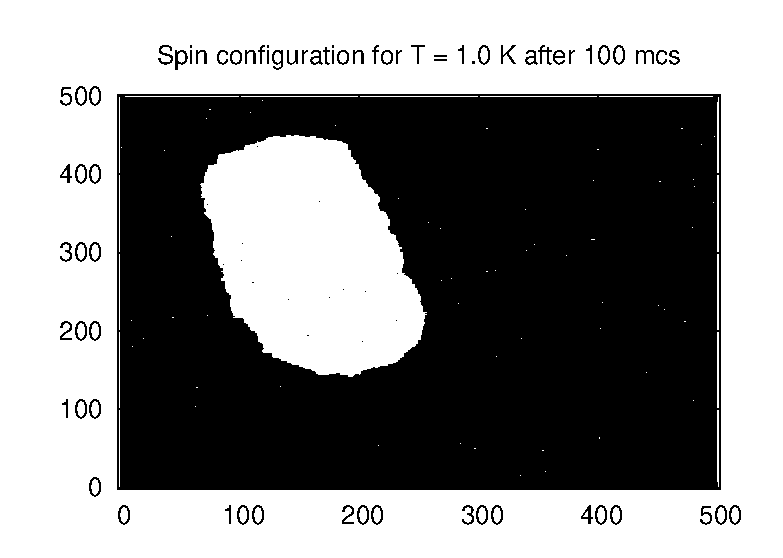
\includegraphics[width=1\textwidth]{cold.eps}
\label{fig:minipage2}
\caption{Metastable state of homogeneous spin regions after 10000 mcs at $T = 1$ K. }
\end{minipage}
\end{figure}

\vspace{3mm}

\begin{figure}[h]
\centering
\begin{minipage}[b]{0.45\linewidth}
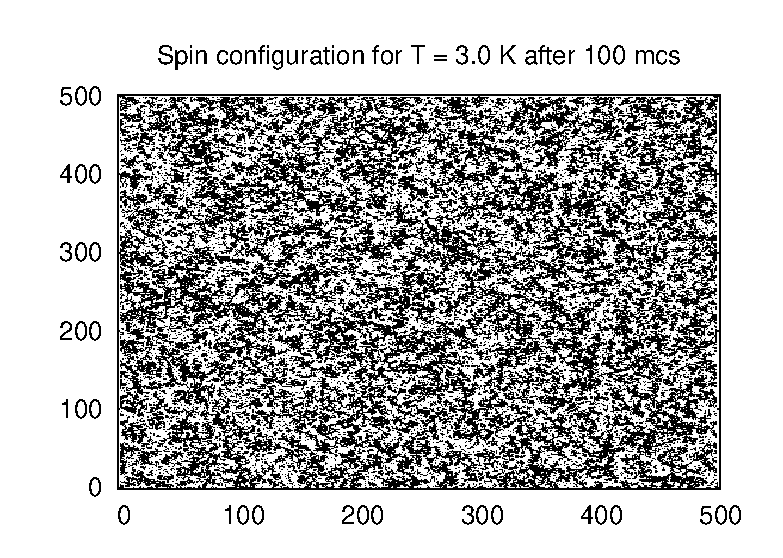
\includegraphics[width=1\textwidth]{warm.eps}
\label{fig:minipage1}
\caption{Random spin configuration in the paramagnetic phase for $T = 3$ K.}
\end{minipage}
\quad
\begin{minipage}[b]{0.45\linewidth}
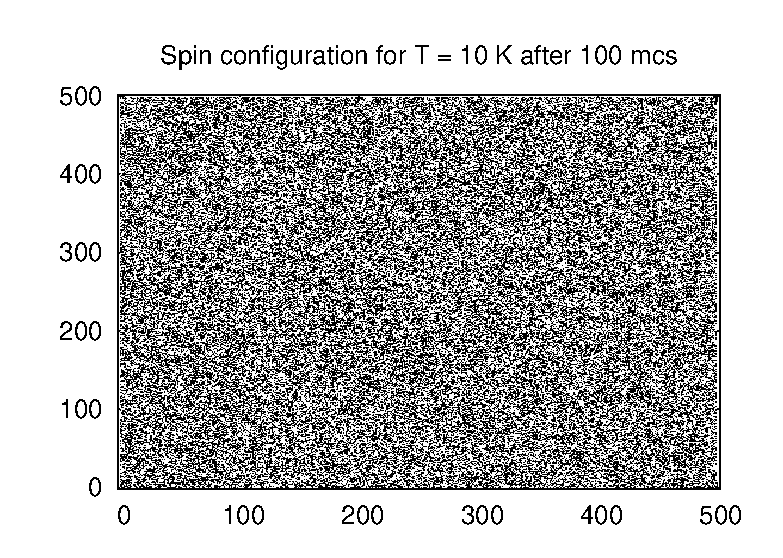
\includegraphics[width=1\textwidth]{hot.eps}
\label{fig:minipage2}
\caption{Checkerboard pattern of antialigned spins for high $T = 10$ K.}
\end{minipage}
\end{figure}

\subsection{Time evolution of the magnetisation}


The time evolution of  $ \langle M \rangle$ for a 25 \small \verb;x; \normalsize 25 lattice was investigated for a range of four initial conditions, (\verb;up;, \verb;down;, \verb;warm; and \verb;hot;), for three temperatures  $T = 0.5, 2.27$ and $5$ K. The number of transients is zeroed. At low temperatures, the starting conditions heavily affect the time evolution of the mean magnetisation. We see from Fig.8 that $ \langle M \rangle$ stabilises to $\pm 1$ depending to the initial spin configuration. On the other hand, for $T \geq T_c$ the plots appear to be independent of the initial conditions. The only difference is the time taken to reach the equilibrium state. As expected, the random configuration minimises the thermalisation steps at intermediate and high T. At low T, the \verb;up; and  \verb;down; configurations take only a few steps to stabilise. At $T_c$, there are large fluctuations in $ \langle M \rangle$ oscillating between the $\pm 1$ extremes (see Fig.10). The net magnetisation disappears (it is zeroed on average) in agreement with the paramagnetic behaviour (see Fig.11) at high T.

\vspace{0.4cm}

\begin{figure}[h]
\centering
\begin{minipage}[b]{0.45\linewidth}
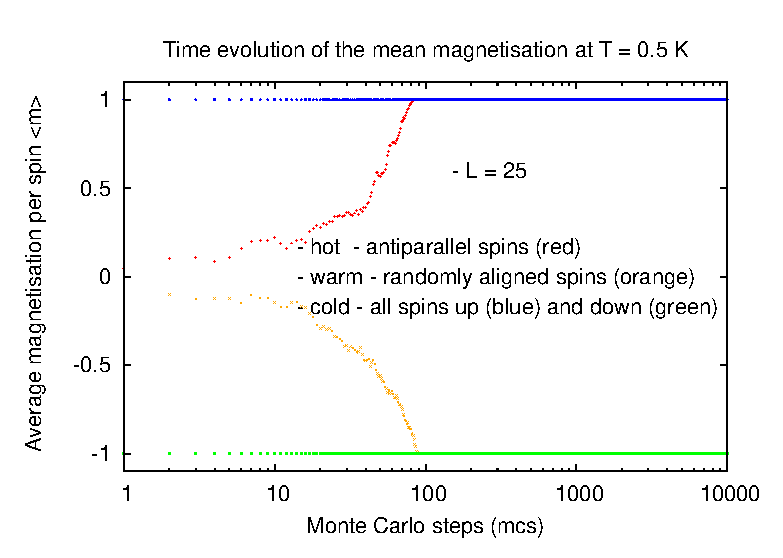
\includegraphics[width=1\textwidth]{subcritical.eps}
\label{fig:minipage1}
\caption{Time evolution of $ \langle M \rangle$ for the four initial conditions (ICs), at $T = 0.5$ K, with $L =25$. If all the spins are already aligned initially then they stabilise in a few steps, but it takes 100 mcs to thermalise for the other ICs.}
\end{minipage}
\quad
\begin{minipage}[b]{0.45\linewidth}
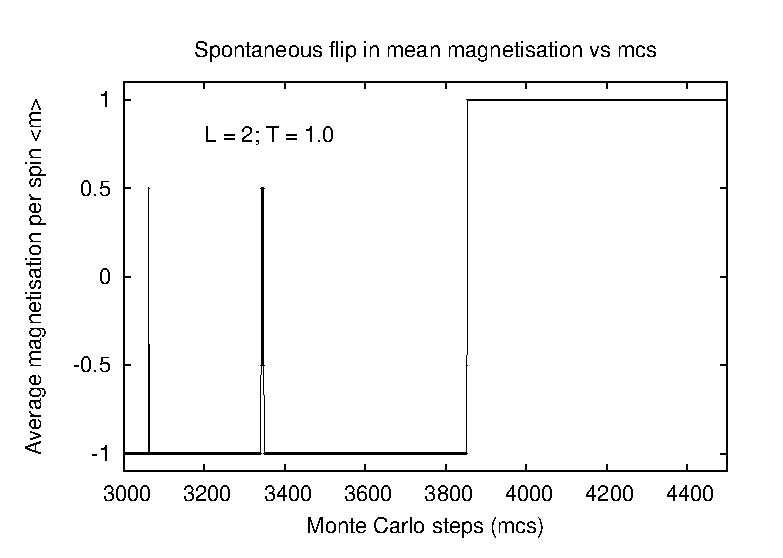
\includegraphics[width=1\textwidth]{flip.eps}
\label{fig:minipage2}
\caption{This figure illustrates a flip in the magnetisation for a 2 x 2 lattice. The occurence of these events is directly proportional to the number of mcs and inversely proportional to lattice size. }
\end{minipage}
\end{figure}

\vspace{1cm}

An interesting feature emerges at low temperatures, the \textit{spontaneous magnetisation}. This is illustrated by Fig.9 for a \small \verb;x; \normalsize lattice at $T = 1.0$ K. It can be shown that, a finite size system cannot have a permanent magnetisation in zero magnetic field. This justifies why sudden flips in the magnetisation can occur for $T <T_c$. Although they are rare, these events will affect the calculation of the mean magnetisation. A sensible solution to minimise these fluctuations is to compute the absolute magnetisation, $ \langle |M| \rangle$, which allows us to consider only a single positive peak.


\begin{figure}[h]
\centering
\begin{minipage}[b]{0.45\linewidth}
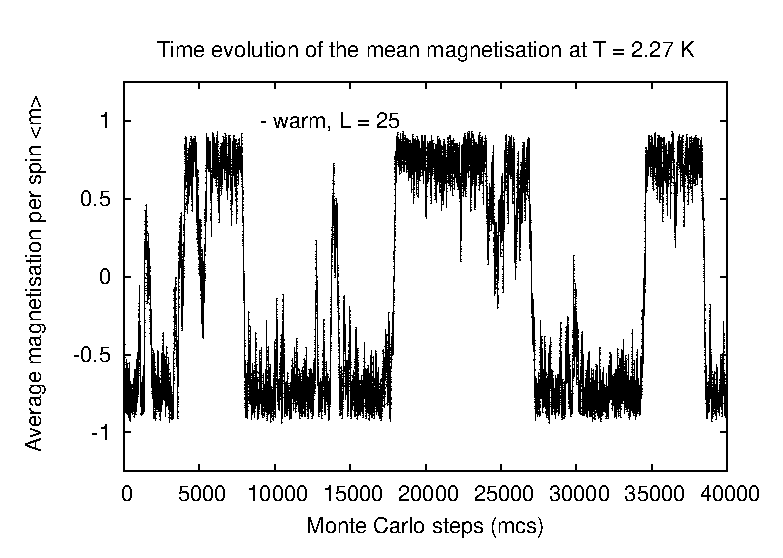
\includegraphics[width=1\textwidth]{critical.eps}
\label{fig:minipage1}
\caption{Time evolution of $ \langle M \rangle$ for random spin initial configuration (warm), at $T = 2.27$ K, with $L =25$. The other ICs all display the same oscillatory pattern.}
\end{minipage}
\quad
\begin{minipage}[b]{0.45\linewidth}
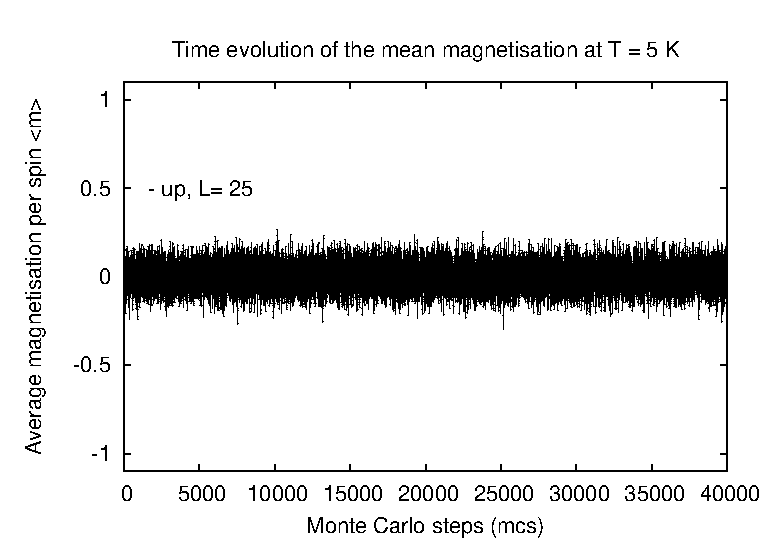
\includegraphics[width=1\textwidth]{supercritical.eps}
\label{fig:minipage2}
\caption{Time evolution of $ \langle M \rangle$ for initially aligned spins (up) at $T = 0.5$ K, with $L =25$. The paramagnetic response is the same for all the ICs.}
\end{minipage}
\end{figure}

\subsection{Magnetisation and energy dependence on temperature}

A valid test of our program is to compare the magnetisation curve at large $L = 50$  against the analytical result derived by Onsanger for the two-dimensional case in the limit $N \rightarrow \infty$ and $H = 0$ \cite{onsanger}. The exact solution for $\langle M \rangle$ is:

\begin{equation}
\langle M \rangle = \lim_{N\to\infty} \frac{\langle \sum_{i} s_i \rangle}{N} = 
\left\{
  \begin{array}{l l}
    [1- \{ sinh(\frac{2}{T}) \}^{-4} ]^{1/8} & \quad \text{for $T_c \leq T$ }\\
     0 & \quad \text{for $T_c > T$}
  \end{array} \right.\
\end{equation}


and is consistent for a considerable range with the $L = 50$ plot (Fig.12). The absolute mean magnetisation $ \langle |M| \rangle$ was plotted to avoid the complications due to spontaneous magnetisation. Both the magnetisation and energy results show that the curves become more pronounced as the lattice size increases. This indicates that the system undergoes the phase transition faster for large $N$. However, in Fig.14 there is not a marked difference between the $L = 8$ and $L= 16$ curve, which could indicate a continuous phase transitions. The critical temperature is shifted as L increases. Fig.13 was used to estimate $T_c = 2.25 \pm 0.05 $ which is compatible with the theoretical value $T_c =  2/ln(1+\sqrt{2}) \approx 2.26918$. The spins are all aligned with stabilised $ \langle E \rangle = -2$ at low T, and randomly aligned at high T, as expected. 


\begin{figure} [H]
\centering
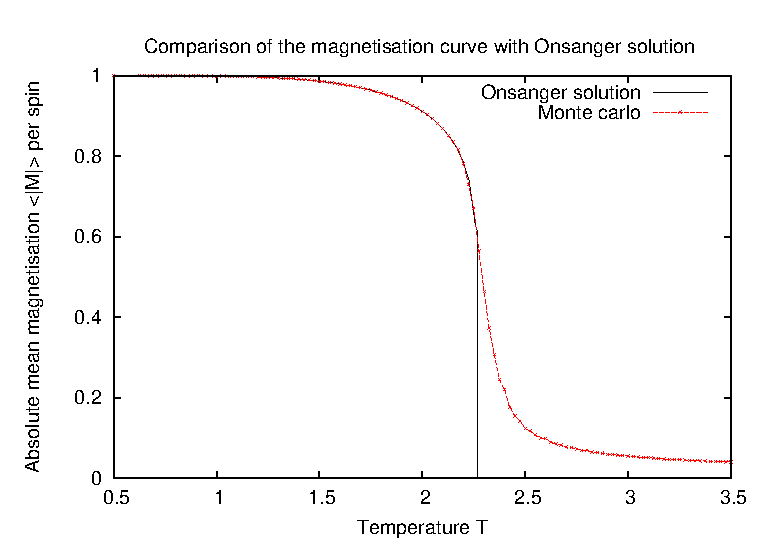
\includegraphics[width=0.6\textwidth]{test.eps}
\caption{\label{fig:generic} This figure illustrates that at large L the numerical solution is consistent with the Onsanger solution. It was used to estimate $T_c = 2.25 \pm 0.05 $ by looking at the point at which the gradient starts falling. }
\end{figure}

\begin{figure} [H]
\centering
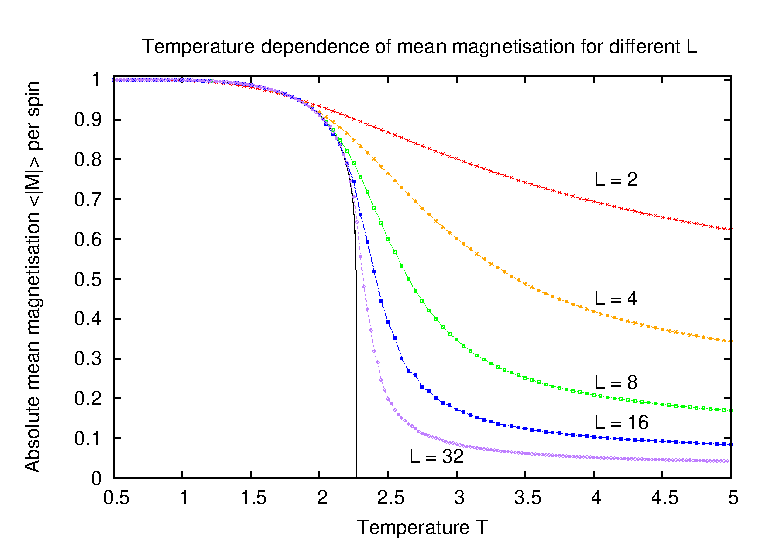
\includegraphics[width=0.6\textwidth]{mag.eps}
\caption{\label{fig:generic} This figure illustrates the slow convergence of the magnetisation curves to Onsanger solution. The random error in $\langle |M| \rangle$ due to the thermal averaging is of the order of one part in a thousand, hence error bars are too small to be displayed on the graph. }
\end{figure}

\begin{figure} [H]
\centering
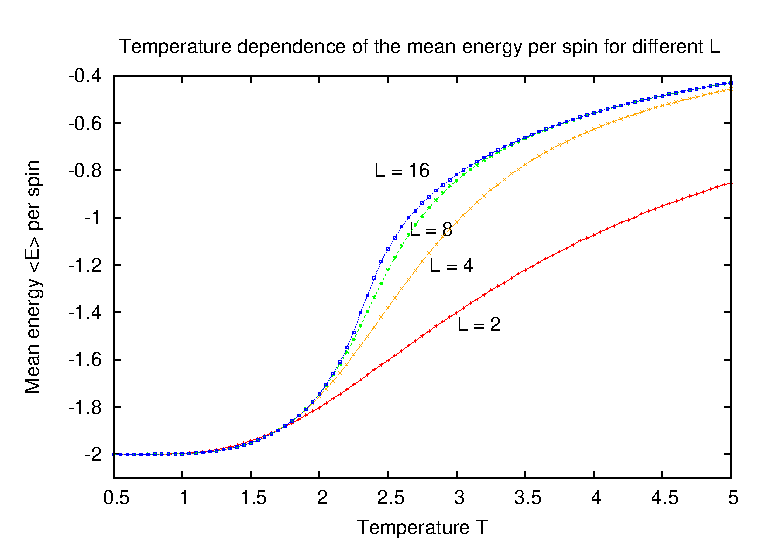
\includegraphics[width=0.6\textwidth]{energy.eps}
\caption{\label{fig:generic} Energy dependence on temperature curves. The curves converge rapidly, indicating a possible continuous phase transition. The error size is the same as in Fig.13, hence error bars are not plotted.}
\end{figure}

\subsection{Heat capacity}

The temperature dependence of the heat capacity C for $L = 2$ was compared with the exact solution to test the numerical method. The analytical estimate of C was used because of its negligible random error. The agreement should improve for larger lattices but these cases are too laborious to compute. There are sixteen possible spin configurations, but exploiting symmetry considerations and degeneracy, they reduce to the four below. 

\begin{figure}[H]
\centering
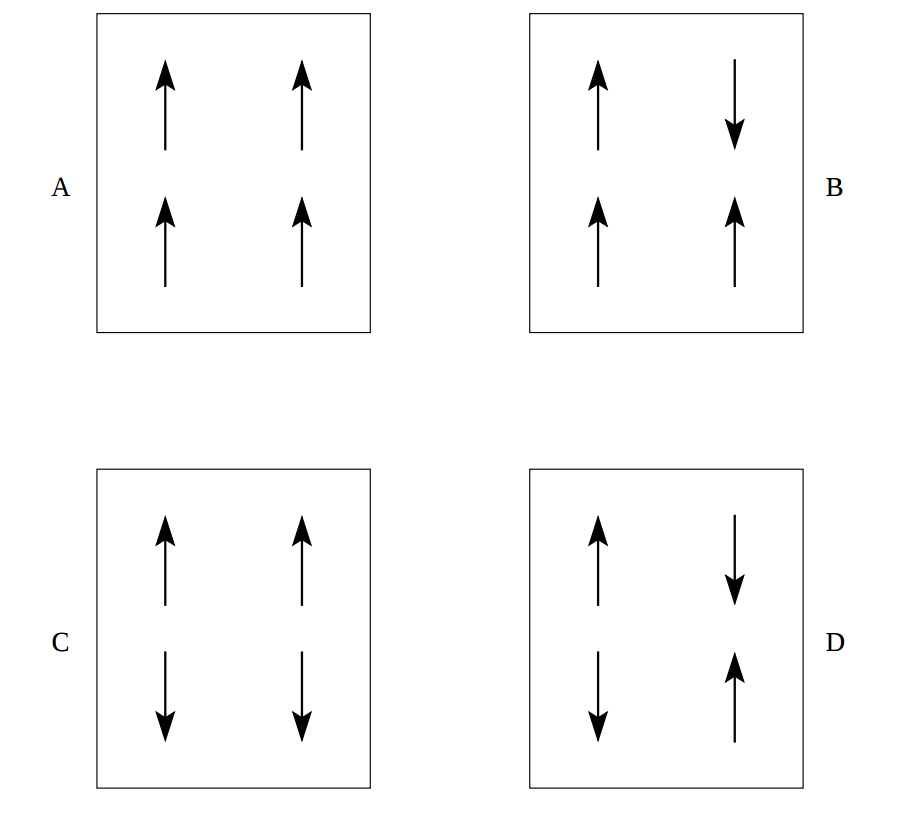
\includegraphics[width=0.35\textwidth]{degeneracy.png}
\label{fig:minipage1}
\caption{The four significant spin configurations for a 2 x 2 lattice.}
\end{figure}

\begin{table} [H]
\centering
\begin{tabular}{|c|c|c|}
\hline
Spin configuration   & Energy(E)      & Degeneracy   \\
\hline
A         &  $-8$ 			  &        2          \\
\hline
B         &  $0$              &        8           \\
\hline
C         &  $0$              &        4          \\
\hline
D         &  $+8$             &        2         \\
\hline
\end{tabular}
\caption{Energies and degeneracies of the spin configuration shown in Fig.15 }
\end{table}

In Table 1, we compute the energy for every configuration and then we calculate the mean and variance of the energy of the system using (3):

\begin{equation}
\langle Z \rangle = 2e^{8 \beta} + 12 + 2e^{-8 \beta}
\end{equation}

\begin{equation}
\langle E \rangle = -\frac{1}{Z} [2(8)e^{8 \beta} + 2(-8)e^{-8 \beta}]
\end{equation}

\begin{equation}
\langle E^2 \rangle = \frac{1}{Z} [2(64)e^{8 \beta} + 2(64)e^{-8 \beta}]
\end{equation}

\begin{figure}[H]
\centering
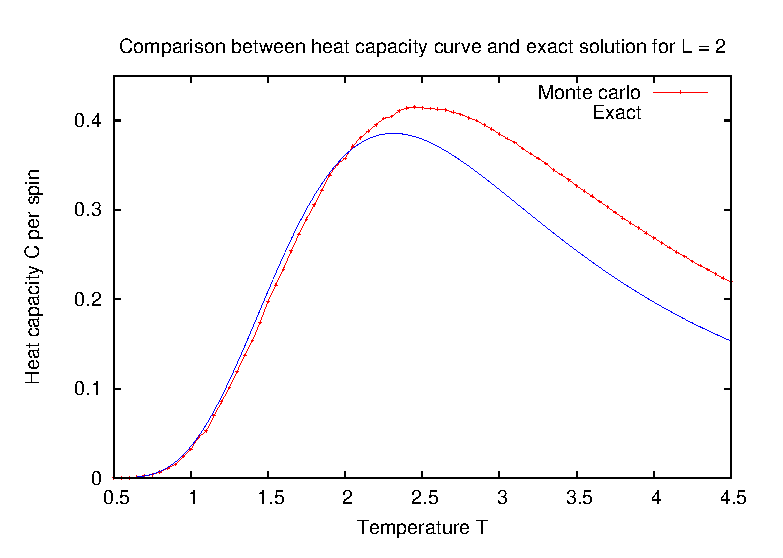
\includegraphics[width=0.6\textwidth]{exact_c.eps}
\label{fig:minipage1}
\caption{Comparison between the numerical and exact solutions of C for $L = 2$.}
\end{figure}

and then we calculate C analytically. This estimate matches extremely well with theory at low temperatures, but starts deviating at the phase transition (Fig.16). The plots of analytic and discrete estimates of C are consistent (Fig.17). The measurement of the latter, however, is dominated by large random errors. The heat capacity peaks at the phase transition as expected. We can improve our estimate for $T_c = 2.29 \pm 0.03 K$ using the $L = 16$ plot.

\begin{figure} [H]
\centering
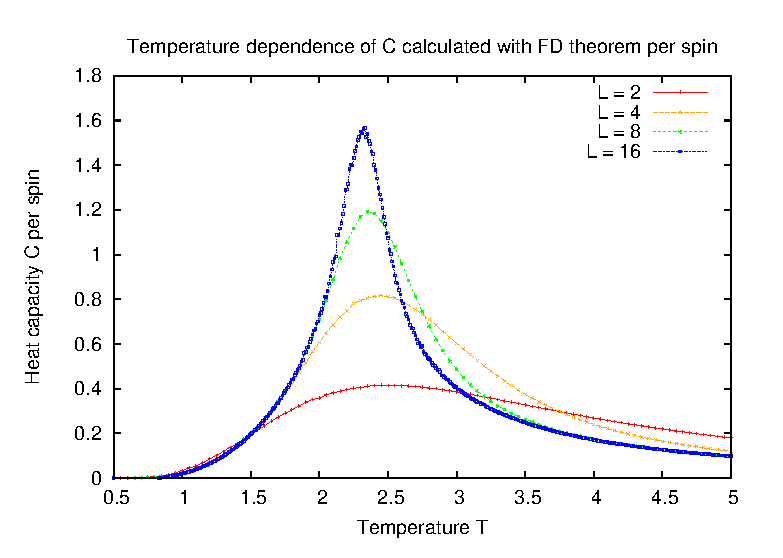
\includegraphics[width=0.6\textwidth]{fluctuation.eps}
\caption{\label{fig:generic} Plot of the temperature dependence of C estimated with the fluctuation dissipation theorem. The error bars are negligible. The peak value of the heat capacity corresponds to the phase transition temperature and was estimated to be $T_c = 2.29 \pm 0.03 K$.}
\end{figure}

\begin{figure} [H]
\centering
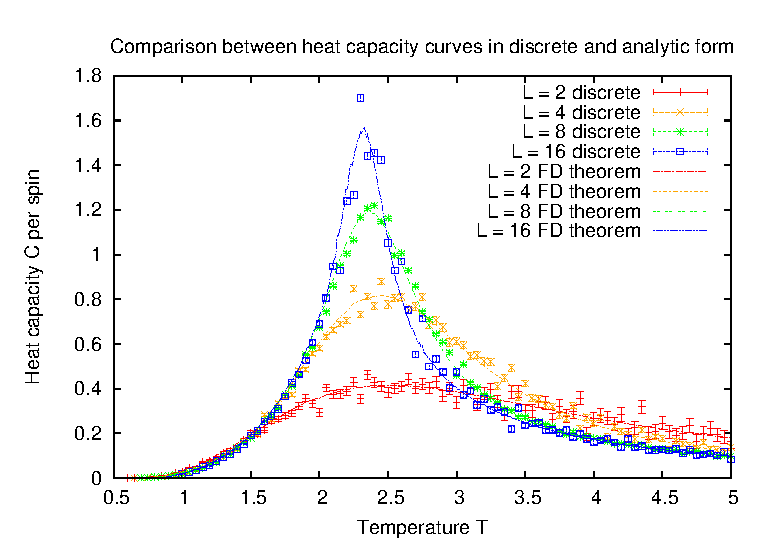
\includegraphics[width=0.6\textwidth]{discrete.eps}
\caption{\label{fig:generic} Plot of the temperature dependence of the discrete form of the heat capacity C. The error bars due to the stochastic error are $\sim 5\%$. The best fit lines are the curves of Fig.17 and show that both estimates are compatible. }
\end{figure}

 \subsection{Finite size scaling}

It becomes useful to define the critical exponent $\beta$, such that $M(T) \sim (T_c -T)^{\beta}$, in order to understand the behaviour of the magnetisation near $T_c$. From theory, we know that $|T-T_c| \ll 1$ as $L \rightarrow \infty$. In particular the critical lattice relation for the two-dimensional case is $(T-T_c)^{-1} \rightarrow L $, hence we find that:

\begin{equation}
 M(T) \sim (T_c -T)^{\beta} \rightarrow L^{-\beta}
 \end{equation}
 
We can determine $\beta$ using linear regression analysis on a log-log plot of the peak value of $M$ close to $T_c$ for different lattice sizes (Fig.19). The value of $\beta$ is simply the modulus of the gradient. This was determined to be $0.126 \pm 0.006$ which is in good agreement with the theoretical value of $1/8$. 

\begin{figure} [H]
\centering
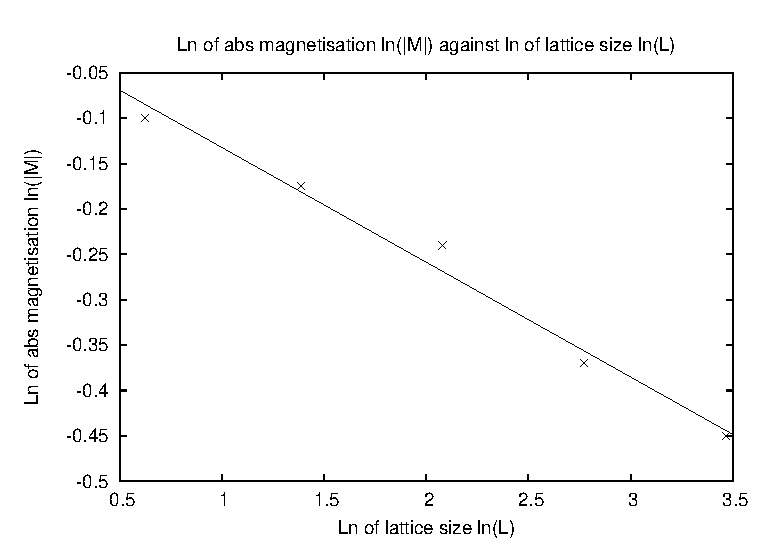
\includegraphics[width=0.6\textwidth]{beta.eps}
\caption{\label{fig:generic}Log-log plot of the absolute mean magnetisation $ \langle |M| \rangle $ against lattice size L. The gradient was found to be $0.126 \pm 0.006$ by means of linear regression analysis. }
\end{figure}

\subsection{The effect of magnetic field on the magnetisation}

The effect of applying an external $H$ field to the $T < T_c$ and $T > T_c$ cases was investigated.  For $T = 2,3$ K, the dependence of $ \langle M \rangle$ on H was plotted for $L = 2,4,16,64$ using a hundred thousands mcs, a thousand transients and step size $\delta H = 0.05$.  Below $T_c$, as we increase $L$ the curves converge to the thermodynamic limit for $L \rightarrow \infty$ of a Heaviside step function (Fig.20). This is due to the fact that for a finite size system a discontinuity cannot occur. Above $T_c$ there is no significant difference between the $L = 32$ and $64$ plots. The convergence to the continuous phase transition in Fig.21 is much more rapid than for low T.   

\begin{figure} [H]
\centering
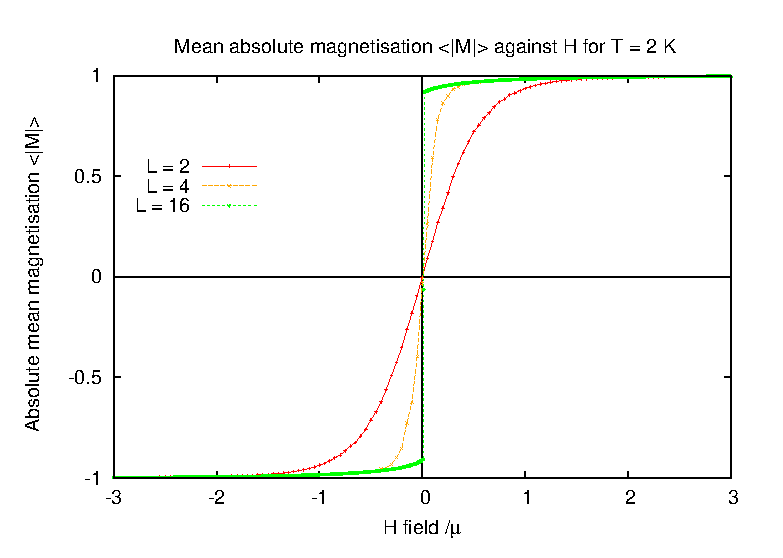
\includegraphics[width=0.6\textwidth]{h_sub.eps}
\caption{\label{fig:generic} Rapid convergence of the magnetisation curves to the discontinuity at $H = 0$ and $T = 2$ K. }
\end{figure}

\begin{figure} [H]
\centering
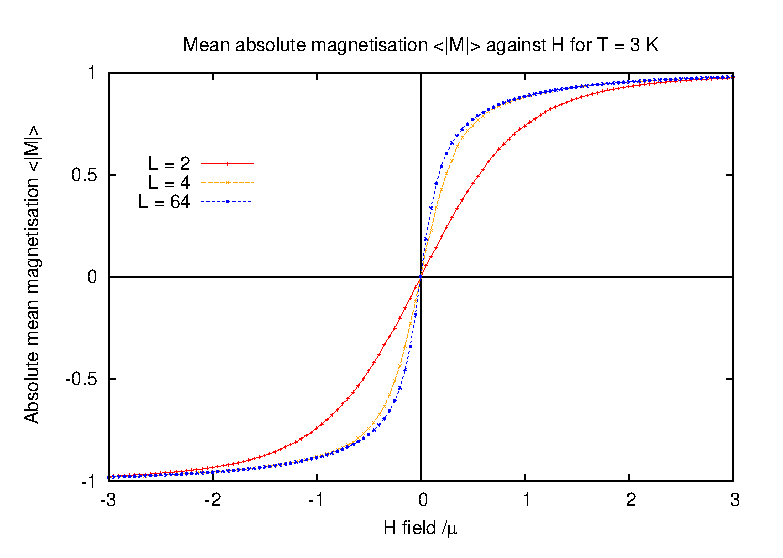
\includegraphics[width=0.6\textwidth]{h_super.eps}
\caption{\label{fig:generic} Slow convergence of the magnetisation curves to the continuous phase transition at $H = 0$ and $T = 3$ K. }\(\)
\end{figure}

\pagebreak

\section {Conclusions}

An analytical solution to the two-dimensional Ising problem is not easily achieved. The problem is far more tractable by using a Monte Carlo simulation with a Metropolis importance sampling technique. The requirement to have accurate results is large lattice size and large number of Monte Carlo steps. The effect of finite lattice size is mitigated by using periodic boundary conditions. The time evolution of the magnetisation was illustrated with suitable spin configurations for a range of initial conditions and temperatures. The frequency of spontaneous magnetisation increases with the number of time steps and decreases with lattice size. In order to overcome this, the absolute mean magnetisation was considered and found to agree in the limit of an infinite lattice size with Onsanger's solution. Temperature dependent plots of $\langle |M| \rangle$ and $\langle E \rangle$ show the occurrence of a continuous phase transition at the critical temperature $T_c$. A better estimate for $T_c = 2.29 \pm 0.03$ was extrapolated from the peak value of the heat capacity $C$ calculated with the fluctuation-dissipation theorem. The other estimate for $C$ in discrete form is consistent but subject to significant random errors. The critical exponent $\beta$ was determined to be $0.126 \pm 0.006$ using finite size scaling. The response of the magnetisation to an applied magnetic field show a discontinuity close to $H = 0$ below $T_c$, and a continuous phase transition for high temperatures. LALAALLALALA

\begin{thebibliography}{3}

\bibitem{stat} J. M. Yeomans \emph{Statistical Mechanics of Phase Transitions}, Clarendon Press, Oxford, 1992.
 \bibitem{mcs} K. Binder and D.W. Heermann. \emph{Monte Carlo Simulation in Statistical Physics}, Springer, Berlin, 1997.
 \bibitem{met} N. Metropolis \emph{The Beginning of the Monte Carlo Method}, Los Alamos Science, No.15, 1987. 
 \bibitem{onsanger} L. Onsager, \emph{Crystal Statistics. I. A Two-Dimensional Model with an Order-Disorder Transition}, Physical Review, 65, 117 (1944).
 
\end{thebibliography}

\appendix

\section{Source code }
\begin{minted}[linenos]{c++}

// Ising Model 2d simulation, computes the observables <|M|>, <E>, C as a function of T

#include <cmath>
#include <cstdlib>
#include <iostream>
#include <fstream>
#include <gsl/gsl_rng.h>

using namespace std;

double J = +1;                              // ferromagnetic coupling
int DimX, DimY;                             // lattice x and y dimensions
int N;                                      // number of spins
int **s;                                    // the spins
double T;                                   // temperature
double minT = 3.5;                          // minimum temperature
double deltaT = 0.01;                       // temperature step size
double H = 0;                               // magnetic field
enum initial_cond {warm, up, down, hot};    // initial spin configurations
int transient = 1000;                       // number of transient steps
double w[17][3];                            // ratio w of transition rates at eq.

// computes random deviate in [0;1]
double rand_uniform( unsigned long int seed = 0 )
 {      static gsl_rng* rng = 0;
        if ( rng == 0 ) rng = gsl_rng_alloc( gsl_rng_default );
        if ( seed != 0 ) gsl_rng_set( rng, seed );
        return gsl_rng_uniform( rng );
}

// precalculates boltzmann factors for fixed T and H
void calc_Boltzmann_factors ( double& T )
{      for (int i = -8; i <= 8; i += 4) {
        w[i + 8][0] = exp( - (i * J + 2 * H) / T);
        w[i + 8][2] = exp( - (i * J - 2 * H) / T);
     }
}

int steps = 0;
initial_cond input;

// initialises spin configuration
void initialise ( ) {
     input = warm;
     s = new int* [DimX];
     for (int i = 0; i < DimX; i++)
          s[i] = new int [DimY];

     // chooses the initial conditions
     for (int i = 0; i < DimX; i++)
     for (int j = 0; j < DimY; j++) {

              if      (input == up)    s[i][j] =  1;
              else if (input == down) s[i][j] = -1;
              else if (input == hot) {
                   if  (((i+j)%2) == 0)
                   s[i][j] = 1;  else  s[i][j] = -1;
                   }
              else s[i][j] = rand_uniform() < 0.5 ? +1 : -1;
              }
         steps = 0;
}

// calculates single Metropolis step
bool Metropolis_step ( ) {

     // chooses a random spin
     int i = int(DimX*rand_uniform());
     int j = int(DimY*rand_uniform());

     // finds its neighbors using periodic boundary conditions
     int iPrev = i == 0 ? DimX-1 : i-1;
     int iNext = i == DimX-1 ? 0 : i+1;
     int jPrev = j == 0 ? DimY-1 : j-1;
     int jNext = j == DimY-1 ? 0 : j+1;

     // finds sum of neighbours
     int sum_neighbours = s[iPrev][j] + s[iNext][j] + s[i][jPrev] + s[i][jNext];
     int delta_ss = 2*s[i][j]*sum_neighbours;

     // ratio of Boltzmann factors
     double ratio = w[delta_ss+8][1+s[i][j]];
     if (rand_uniform() < ratio) {
          s[i][j] = -s[i][j];
          return true;
     } else return false;
}

double acceptance_ratio;

// single Monte carlo step per spin
void single_mcs_per_spin ( ) {
     int accepts = 0;
     for (int i = 0; i < N; i++)
          if (Metropolis_step())
               ++accepts;
     acceptance_ratio = accepts/double(N);
     ++steps;
}

// prints the spin configuration in binary code
void print_spin_config( )  {
     ofstream file("spin_configuration.data");
     for (int i = 0; i < DimX; i++) {
     for (int j = 0; j < DimY; j++)
          { file << (s[i][j]+1)/2 << " ";
          } file << '\n';
     }
      file.close();
}

// calculates the magnetisation per spin
double magnetisation_per_spin ( ) {
     int sSum = 0;
     for (int i = 0; i < DimX; i++)
     for (int j = 0; j < DimY; j++) {
          sSum += s[i][j];
     }
     return -sSum / double(N);
}

// calculates the energy per spin
double energy_per_spin ( ) {
     int sSum = 0, ssSum = 0;
     for (int i = 0; i < DimX; i++)
     for (int j = 0; j < DimY; j++) {
          sSum += s[i][j];
          int iNext = i == DimX-1 ? 0 : i+1;
          int jNext = j == DimY-1 ? 0 : j+1;
          ssSum += s[i][j]*(s[iNext][j] + s[i][jNext]);
     }
     return -(J*ssSum + H*sSum)/N;
}

int main (int argc, char *argv[]) {

     cout << " 2d Ising Model, Monte Carlo - Metropolis simulation \n"
          << " ---------------------------------------------------\n"
          << " Enter lattice size L: ";
     cin >> DimX;
     DimY = DimX;
     N = DimX*DimY;
     cout << " Enter number of mcs: ";
     int mcs;
     cin >> mcs;

     // initialises summation of variables and errors at each step
      double Mmed = 0, Mvar = 0, Emed = 0, Evar = 0, Mabs = 0, Ebef = 0;
      double errE = 0, errM = 0, errC = 0, errEbef = 0;

     initialise();
     ofstream file("temperature_loop.data");

     // temperature loop
     for(T = minT; T < 5 ; T += deltaT )
     {
            calc_Boltzmann_factors (T);
            Ebef = Emed;
            errEbef = errE;

            // transient function
            for (int s = 0; s < transient; s++)
                single_mcs_per_spin();

            // Montecarlo loop
            for (int t = 0; t < mcs; t++) {
                single_mcs_per_spin();
                double m = magnetisation_per_spin();
                double e = energy_per_spin();

                // keeps summation of observables
                Mmed += m; Mvar += m * m;
                Emed += e; Evar += e * e;
                Mabs += sqrt(m * m);
                }

        //average observables
        Mmed /= mcs; Mvar /= mcs;
        Emed /= mcs; Evar /= mcs;
        Mabs /= mcs;

        //error calculation for <E>, <|M|>, and C (discrete derivative)
        errE = sqrt((Evar - Emed * Emed)/mcs);
        errM = sqrt((Mvar - Mmed * Mmed)/mcs);
        errC = sqrt( errE * errE + errEbef * errEbef )/deltaT;

        // outputs results to file
        file <<   T   << "\t" <<                       //  temperature
        "\t" <<  Emed << "\t" << errE <<               //  <E> per spin with error
        "\t" <<  Mabs << "\t" << errM <<               //  <|M|> per spin with error
        "\t" <<  (Evar - (Emed * Emed ))*N/(T*T) <<    //  C per spin (fluct-dissip theorem)
        "\t" <<  (Emed - Ebef)/deltaT   <<             //  C per spin (discrete derivative)
        "\t" <<  errC <<  endl;                        //  and its error

        }
       file.close();
}

}
\end{minted}

\begin{minted}[linenos]{c++}

// ising2.cc computes <|M|> as a function of H

#include <cmath>
#include <cstdlib>
#include <iostream>
#include <fstream>
#include <gsl/gsl_rng.h>

using namespace std;

double J = +1;                  // ferromagnetic coupling
int DimX, DimY;                 // lattice x annd y dimensions
int M;                          // number of spins
int **s;                        // the spins
double T;                       // temperature
double Hmax = 3.0;              // maximum magnetic field
double dH = 0.005;              // field step size
double w[17][3];                // ratio w of transition rates at eq.
int transient_steps = 1000;     // transient steps

// computes random deviate in [0;1]
double rand_uniform( unsigned long int seed = 0 )
 {      static gsl_rng* rng = 0;
        if ( rng == 0 ) rng = gsl_rng_alloc( gsl_rng_default );
        if ( seed != 0 ) gsl_rng_set( rng, seed );

        return gsl_rng_uniform( rng );
}

// precalculates boltzmann factors for fixed T and H
void calc_Boltzmann_factors ( double& H ) {
     for (int i = -8; i <= 8; i += 4) {
          w[i + 8][0] = exp( - (i * J + 2 * H) / T);
          w[i + 8][2] = exp( - (i * J - 2 * H) / T);
     }
}

int steps = 0;                  // steps so far

// initialises a random spin configuration
void initialize ( ) {
     s = new int* [DimX];
     for (int i = 0; i < DimX; i++)
          s[i] = new int [DimY];
     for (int i = 0; i < DimX; i++)
          for (int j = 0; j < DimY; j++)
               s[i][j] = rand_uniform() < 0.5 ? +1 : -1;
     steps = 0;
}

// computes single Metropolis step per spin
bool Metropolis_step ( ) {

     // chooses a random spin
     int i = int(DimX*rand_uniform());
     int j = int(DimY*rand_uniform());

     // finds its neighbors using periodic boundary conditions
     int iPrev = i == 0 ? DimX-1 : i-1;
     int iNext = i == DimX-1 ? 0 : i+1;
     int jPrev = j == 0 ? DimY-1 : j-1;
     int jNext = j == DimY-1 ? 0 : j+1;

     // finds sum of neighbours
     int sum_neighbours = s[iPrev][j] + s[iNext][j] + s[i][jPrev] + s[i][jNext];
     int delta_ss = 2*s[i][j]*sum_neighbours;

     // computes ratio of Boltzmann factors
     double ratio = w[delta_ss+8][1+s[i][j]];
     if (rand_uniform() < ratio) {
          s[i][j] = -s[i][j];
          return true;
     } else return false;
}

double acceptance_ratio;

// computes single Monte Carlo step per spin
void single_mcs_per_spin ( ) {
     int accepts = 0;
     for (int i = 0; i < M; i++)
          if (Metropolis_step())
               ++accepts;
     acceptance_ratio = accepts/double(M);
     ++steps;
}

// calculates the mean magnetisation per spin
double magnetization_per_spin ( ) {
     int sSum = 0;
     for (int i = 0; i < DimX; i++)
     for (int j = 0; j < DimY; j++) {
          sSum += s[i][j];
     }
     return -sSum / double(M);
}


int main (int argc, char *argv[]) {

     cout << " Ising 2d Model - Monte Carlo Metropolis simulation\n"
          << " ---------------------------------------------------\n"
          << " Enter lattice size: ";
     cin >> DimX;
     DimY = DimX;
     M = DimX*DimY;
     cout << " Enter temperature T: ";
     cin >> T;
     cout << " Enter number of mcs: ";
     int mcs;
     cin >> mcs;
     double Mmed = 0, Mvar = 0, Mabs = 0, H = 0;

     initialize();
     ofstream file("hfield_response.data");

     // magnetic field loop
      for (H =-Hmax; H <= Hmax; H += dH )
     {
          calc_Boltzmann_factors( H );

          // transient function
          for (int s = 0; s < transient_steps; s++)
          single_mcs_per_spin();

            // Monte Carlo loop
            for (int s = 0; s < mcs; s++)
            {
             single_mcs_per_spin();

             // sum of total magnetisation
             double m = magnetization_per_spin();
             Mmed += m; Mvar += m * m;
             Mabs += sqrt(m* m);
            }

     // finds <|M|> and outputs it and H to a file
     Mmed /= mcs;
     file << H << "\t" << Mmed << endl;
     }
    file.close();
}

\end{minted}



\end{document}
